\chapter{Experiments}\label{chapter:experiments}

\section{Datasets}
We use the following datasets for our experiments (as well as synthetic data). 
\begin{itemize}
    \item Iris dataset \cite{iris_dataset}
    \item MNIST \cite{mnist_dataset}
    \item EMNIST letters \cite{emnist_dataset}
    \item flow cytometry \cite{flow_dataset}
    \item Macasko mouse retina \cite{Macosko_dataset} 
\end{itemize}

\section{Dataset Cluster Assumptions}
Here we investigate if assumptions made for clustering results in \cite{LinStei22} hold in practice, by looking at the simple Iris dataset. 
The reason that we look at Iris is that it is a very small dataset, which makes it feasible to look at all $N^2 = 150^2$ affinities $p_{ij}$ individually.  

Recalling \ref{eq:4.1}, we make the assumption that the data we perform t-SNE on is clustered. 
A natural question to ask then is: does real-life data that looks clustered to us humans fulfill this definition of clustered that is required: 
\begin{equation}
    p_{ij} \geq \frac{1}{10 N |\Omega(i)|}
\end{equation}
for all pairs of points $x_i, x_j$ that lie in the same cluster $\Omega(i)$? 

In order to investigate this question, we chose the Iris dataset. 
Ordering the data points in terms of cluster membership (there are 50 points of each of the three clusters), we can visualize what the high-dimensional similarity values $p_{ij}$ look like when using the standard parameters (perplexity = 30). 

\begin{figure}[h]
    %\begin{center}
    \centering 
        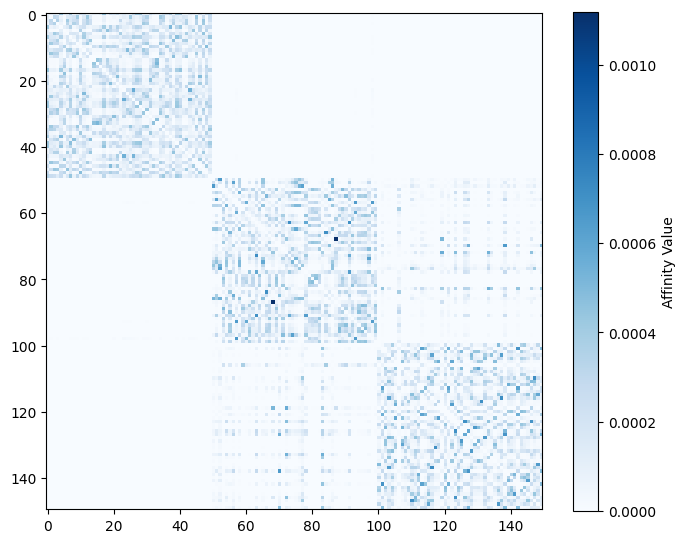
\includegraphics[width=0.7\linewidth]{figures/iris_affinity_matrix.png}
        \caption{Affinity values $p_{ij}$ of the Iris dataset visualized. The affinity matrix was generated using the standard perplexity value of 30.}
    %\end{center}
    \label{fig:iris_affinities}
\end{figure}

We can see the three clusters of the Iris dataset pretty clearly. 
From the visualization \ref{fig:iris_affinities}, it also seems like the first cluster is more well-defined than the second and third are. 
\textcolor{red}{If we run a dimensionality algorithm like PCA or t-SNE on it, we can also see that it performs well and clearly separates at least the first cluster from the other two.} 

So, it would seem that at least this first cluster would fulfil the condition that \begin{equation} p_{ij} \geq \frac{1}{10 N |\Omega(i)|} = \frac{1}{10 \cdot 150 \cdot 50} \end{equation}

However, when we investigate the $p_{ij}$ values of the first cluster (excluding, of course, the diagonal elements, since they are always zero), we notice that the smallest $p_{ij}$ value we observe is (rounded) $2.8 \cdot 10^{-7}$, whereas we calculated a lower bound of about $1.3 \cdot 10^{-5}$ above.
Furthermore, we calculated that a total number of 354 similarites between points in this same first cluster are smaller than the minimal $p_{ij}$ value required for it to be a cluster. 
Now, while \cite{LinStei22} do mention that there is some flexibility with respect to the exact constant being used - we would have to increase it by two orders of magnitude for this result to hold. 

For the last two clusters, we observe something even more interesting. 
If we consider the second cluster, we see that that the smallest similarity value between two points in it is $0.0$. 
This makes it virtually impossible to consider as a cluster, not matter how far we would scale the constant. 
One might argue that indeed clusters 2 and 3 belong together, but also then we observe some points having $0$ similarity to each other. 

\section{Initialization}
Here we reproduce results from \cite{kobak21} on synthetic data and show that t-SNE with PCA initialization can reconstruct geometric shapes up to some extent. 

We also investigate the effects of PCA initialization on real-world datasets. 

\section{An Implementation of Rescaled t-SNE for Large Data Limits}
something here 

\section{Effect of Varying Perplexity Values}
there were some figures here before I removed them. 

\section{Early Exaggeration}
what effect does it have? 

\section{opt-SNE Implementation}
and comparison to default settings 